\documentclass{article}


\usepackage{graphicx} % Required for inserting images

\title{Project-1 Report: Arbitrary-Precision Arithmetic in Java}
\author{Chakram Siri - CS24BTECH11017}
\date{}

\begin{document}

\maketitle

\section{Introduction}
This project implements arbitrary-precision arithmetic operations on integers and floating-point numbers using object-oriented principles in Java. It supports operations such as addition, subtraction, multiplication, and division on numbers of theoretically unlimited size and precision.

\section{Design}
The following design principles were applied during the development of this arbitrary-precision arithmetic system:
\begin{itemize}
    \item \textbf{AFloat:}
    The \texttt{AFloat} is composed of two objects: integral and fractional.Decimal alignment is handled manually during operations to preserve arbitrary precision.

    \item \textbf{Parsing and Input Validation:}
    The parse methods in \texttt{AInteger} and \texttt{AFloat} convert string input to internal object representations.
    
    \item \textbf{Separation of Integer and Floating-Point Arithmetic:} 
    The library distinguishes between integer and floating-point numbers. The \texttt{AInteger} class is designed to handle operations for integers, and the \texttt{AFloat} class is designed to handle floating-point numbers. 
    
    \item \textbf{Arbitrary-Precision Arithmetic:}
    Both classes \texttt{AInteger} and \texttt{AFloat} store the numbers as strings, representing them digit by digit. This allows for arbitrary precision, meaning the library can handle numbers with as many digits as needed. The main operations, such as addition, subtraction, multiplication, and division, are implemented manually by iterating through the digits of the numbers.


    \item \textbf{Support for Basic Operations:} 
    The core arithmetic operations (addition, subtraction, multiplication, and division) are supported for both integer and floating-point numbers. These operations are designed to work for numbers with arbitrary precision, and special care is taken to handle edge cases, such as division by zero, and to ensure correct rounding for floating-point operations.

    \item \textbf{Utility Methods:}
    Several utility methods are included in both classes to assist with parsing, negation, padding, and truncation. For example, the \texttt{padRight} and \texttt{padLeft} methods ensure that the fractional and integer parts of numbers are aligned properly during arithmetic operations. The \texttt{truncateDecimalPlaces} method is used in the \texttt{AFloat} class to limit the number of decimal places for non-terminating decimals.

    \item \textbf{Seamless Integration:} 
    The \texttt{MyInfArith} class acts as the entry point for the program, allowing the user to specify the type of arithmetic (integer or floating-point) and the operation (addition, subtraction, multiplication, or division). The program takes the input from the user, processes it, and outputs the result in the same arbitrary precision format.


\end{itemize}

\begin{figure}[H]
    \centering
    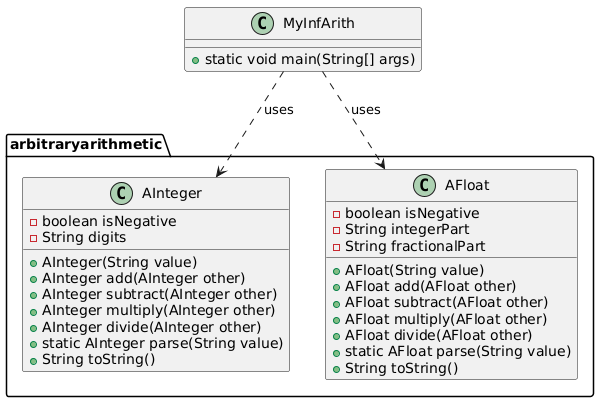
\includegraphics[width=0.8\textwidth]{image.png} % Placeholder for UML diagram
    \caption{UML Class Diagram for the Arbitrary Precision Arithmetic Library}
    \label{fig:uml}
\end{figure}

\end{document}
